\documentclass{beamer}

\usepackage[utf8]{inputenc}
\usepackage[portuguese]{babel}
\usepackage{graphicx}
\usepackage{tikz}
\usepackage{hyperref}
\usepackage{lipsum}

\usepackage{./libs/solarized-light}

\usetheme{Luebeck}

\title{Curso de Plone}
\author{Rodrigo Ferreira de Souza}
\date{Outubro de 2019}

\usebackgroundtemplate{%
    \tikz\node[opacity=0.2] {
        \vbox to \paperheight{
            \vspace{14mm}
            \vfil
            \hbox to \paperwidth{
                \hfil
                
\includegraphics[height=.6\paperheight]{./img/background.png}
                \hfil
            }
            \vfil
        }
    };
}
\hypersetup{
    colorlinks=true,
    linkcolor=cyan,
    filecolor=magenta,      
    urlcolor=blue,
}

\begin{document}

\maketitle

\AtBeginSection[] {
  \begin{frame}
    \frametitle{Onde estamos}
    \tableofcontents[currentsection]
  \end{frame}
}

\section{Usando o Plone}
\subsection{O que é o Plone CMS?}
\begin{frame}
    \frametitle{O que é o Plone CMS?}
    \begin{itemize}
        \item Plone lida com a navegação, publicação e design - te permite focar no conteúdo
        \item Mais controle sobre o conteúdo
        \begin{itemize}
            \item Quem possui acesso
            \item Mantém histórico das versões anteriores
        \end{itemize}
        \item \href{https://plone.com/try-plone.html}{Experimente o Plone}
    \end{itemize}

    Exemplos de sites com Plone são:
    \newline
    \href{https://www.gov.br}{Governo Brasileiro}
\end{frame}

\subsection{Estrutura de pastas}
\begin{frame}
    \frametitle{Estrutura de pastas}
    \begin{figure}
        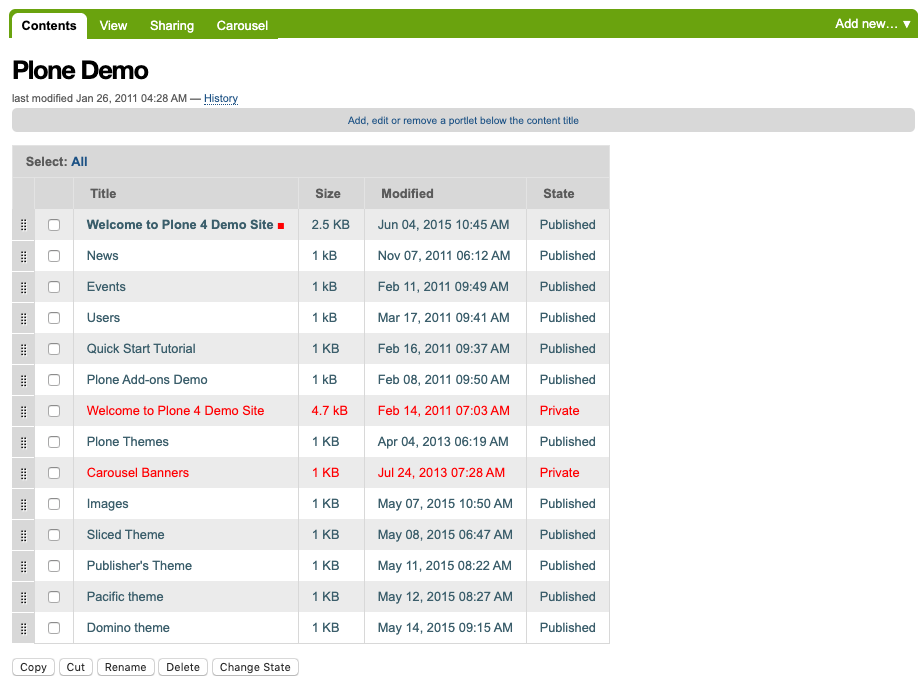
\includegraphics[width=.7\textwidth]{./img/001-001_-_folder.png}
        \caption{Listagem de pastas do Plone}
    \end{figure}
\end{frame}

\subsection{Criar páginas}
\begin{frame}
    \frametitle{Criar páginas}
    \begin{figure}
        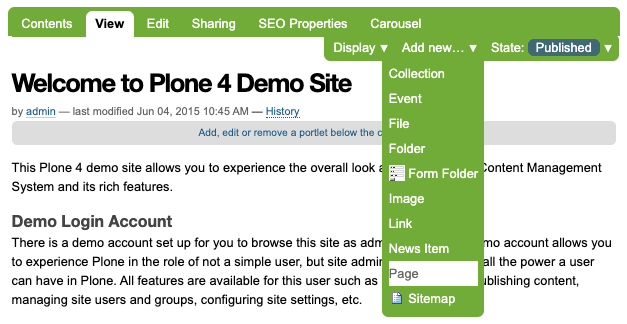
\includegraphics[width=.7\textwidth]{./img/001-002_-_create_page.png}
        \caption{Menu para criação de páginas}
    \end{figure}
\end{frame}

\subsection{Adicionar texto}
\begin{frame}
    \frametitle{Adicionar texto}
    \begin{figure}
        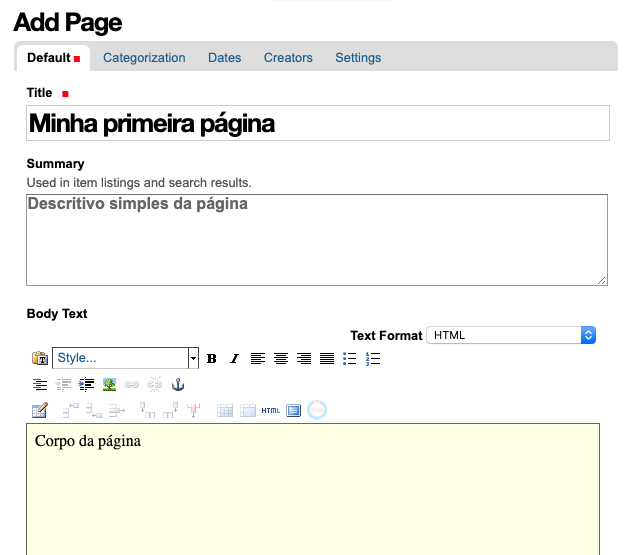
\includegraphics[height=.7\textheight]{./img/001-003_-_adicionar_texto.png}
        \caption{Redigindo uma página}
    \end{figure}
\end{frame}

\subsection{Publicar}
\begin{frame}
    \frametitle{Publicar}
    \begin{figure}
        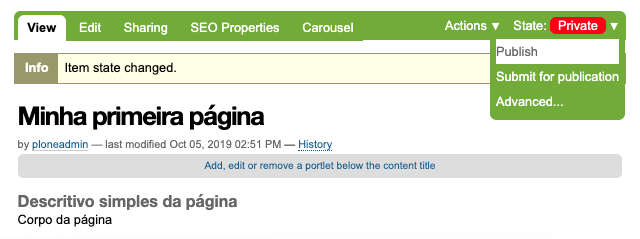
\includegraphics[width=.7\textwidth]{./img/001-004_-_publicar_pagina.png}
        \caption{Workflow simples - Publicar página}
    \end{figure}
\end{frame}

\subsection{Página publicada}
\begin{frame}
    \frametitle{Página publicada}
    \begin{figure}
        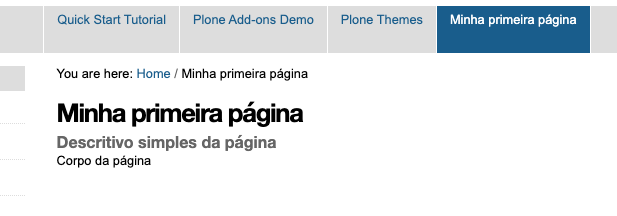
\includegraphics[width=.7\textwidth]{./img/001-005_-_pagina_publicada.png}
        \caption{Resultado final}
    \end{figure}
\end{frame}

\subsection{portlets}
\begin{frame}
    \frametitle{portlets}
    \begin{figure}
        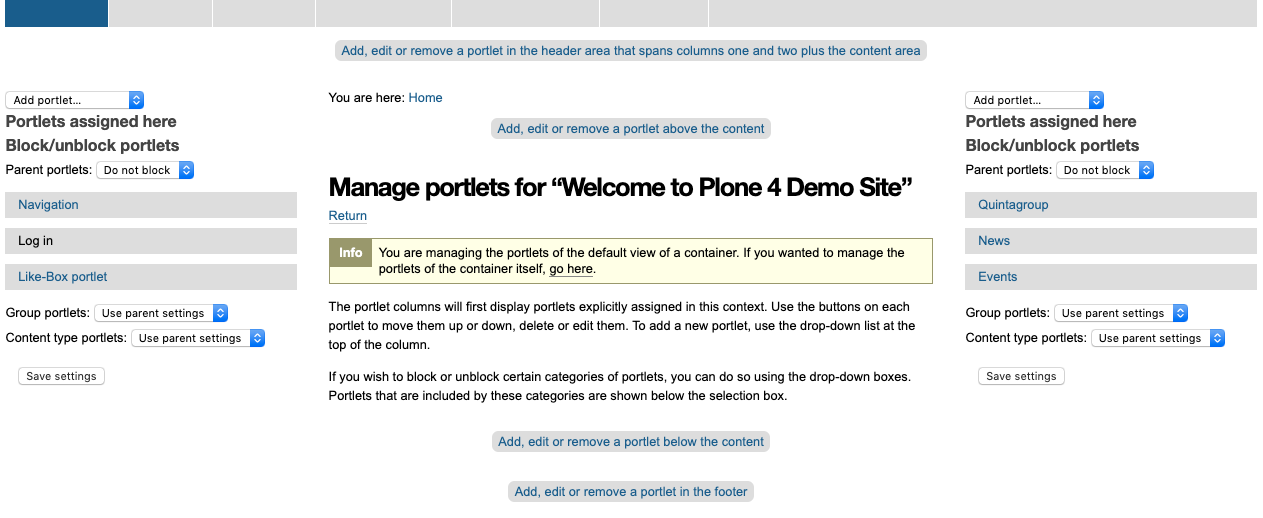
\includegraphics[width=.7\textwidth]{./img/001-006_-_portlets.png}
        \caption{gerenciador de portlets}
    \end{figure}
\end{frame}

\section{IDG - Identidade Digital de Governo}
\subsection{Portal Padrão}
\begin{frame}
    \frametitle{Portal Padrão}
    \begin{figure}
        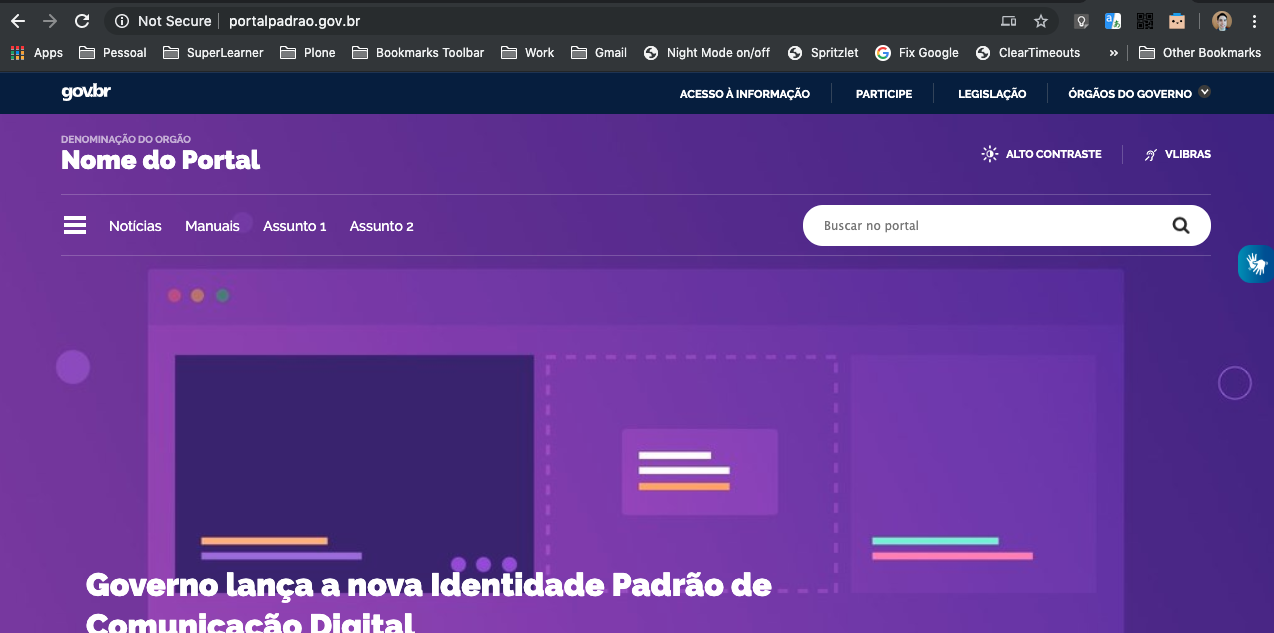
\includegraphics[width=.7\textwidth]{./img/001-007_-_portal_padrao.png}
        \caption{\href{http://www.portalpadrao.gov.br/}{Site do Portal Padrão}}
    \end{figure}
\end{frame}

\subsection{Características}
\begin{frame}
    \frametitle{Características}
    \begin{columns}
        \column{.4\textwidth}
        Temas que seguem \href{http://emag.governoeletronico.gov.br/}{eMAG}
        \begin{itemize}
            \item \href{https://github.com/plonegovbr/brasil.gov.portal}{brasil.gov.portal} \pause
            \item \href{https://github.com/plonegovbr/brasil.gov.temas}{brasil.gov.temas} \pause
            \item \href{https://github.com/plonegovbr/brasil.gov.portlets}{brasil.gov.portlets} \pause
            \item \href{https://github.com/plonegovbr/brasil.gov.tiles}{brasil.gov.tiles} \pause
            \item \href{https://github.com/plonegovbr/brasil.gov.barra}{brasil.gov.barra} \pause
            \item \href{https://github.com/plonegovbr/brasil.gov.agenda}{brasil.gov.agenda} \pause
            \item \href{https://github.com/plonegovbr/brasil.gov.vcge}{brasil.gov.vcge}
        \end{itemize}

        \column{.3\textwidth}
        Complementos
        \begin{itemize}
            \item \href{https://github.com/collective/collective.cover}{Cover} \pause
            \item \href{https://github.com/collective/collective.fingerpointing}{Finger Pointing} \pause
            \item \href{https://github.com/collective/collective.lazysizes}{Lazy Sizes} \pause
            \item \href{https://github.com/collective/collective.liveblog}{Live Blog} \pause
            \item \href{https://github.com/collective/collective.nitf}{NITF} \pause
        \end{itemize}
        \column{.3\textwidth}
        \begin{itemize}
            \item \href{https://github.com/collective/collective.polls}{Polls} \pause
            \item \href{https://github.com/collective/collective.upload}{Upload} \pause
            \item \href{https://github.com/collective/sc.social.likes}{Likes} \pause
            \item \href{https://github.com/collective/sc.photogallery}{Photogallery} \pause
            \item \href{https://github.com/collective/sc.embedder}{Embedder}
        \end{itemize}
    \end{columns}
\end{frame}

\subsection{Cover}
\begin{frame}
    \frametitle{Cover}
    \begin{figure}
        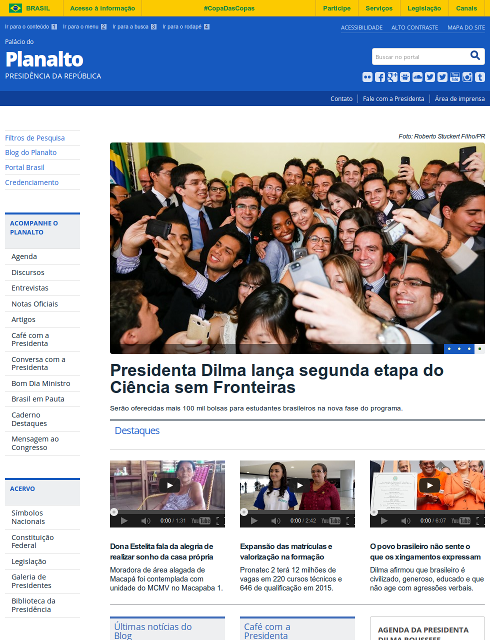
\includegraphics[height=.7\textheight]{./img/001-008_-_cover.png}
        \caption{\href{https://github.com/collective/collective.cover/blob/master/docs/end-user.rst}{Tutorial para usuários}}
    \end{figure}
\end{frame}

\subsection{Upload}
\begin{frame}
    \frametitle{Upload}
    \begin{figure}
        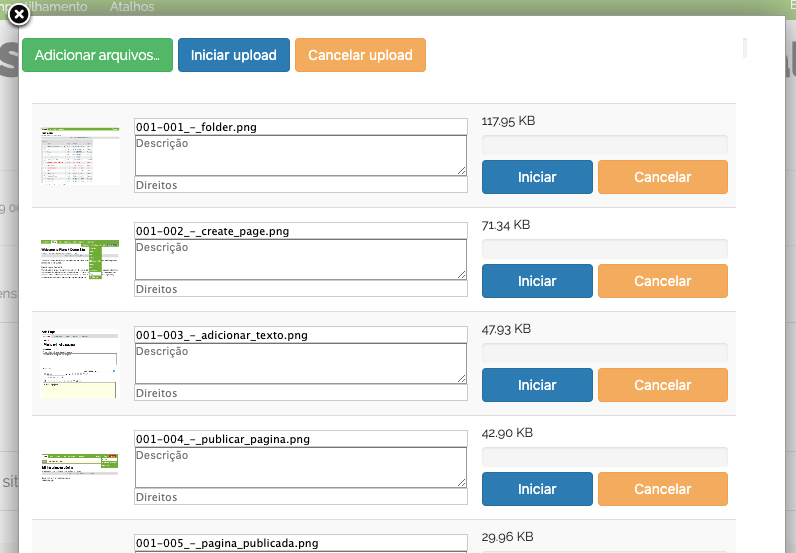
\includegraphics[height=.7\textheight]{./img/001-009_-_upload.png}
        \caption{\href{https://github.com/collective/collective.upload}{Collective Upload}}
    \end{figure}
\end{frame}

\subsection{NITF e Likes}
\begin{frame}
    \frametitle{NITF e Likes}
    \begin{figure}
        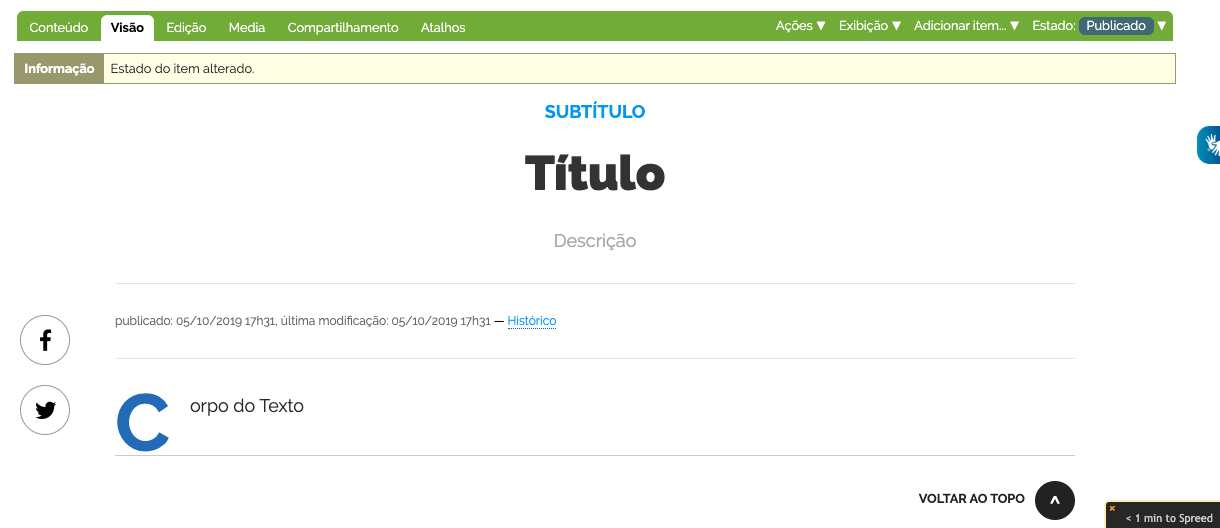
\includegraphics[height=.6\textheight]{./img/001-010_-_nitf_e_likes.png}
        \caption{\href{https://github.com/collective/collective.nitf}{NITF} e \href{https://github.com/collective/sc.social.likes}{Likes}}
    \end{figure}
\end{frame}

\subsection{Embedder}
\begin{frame}
    \frametitle{Embedder}
    \begin{figure}
        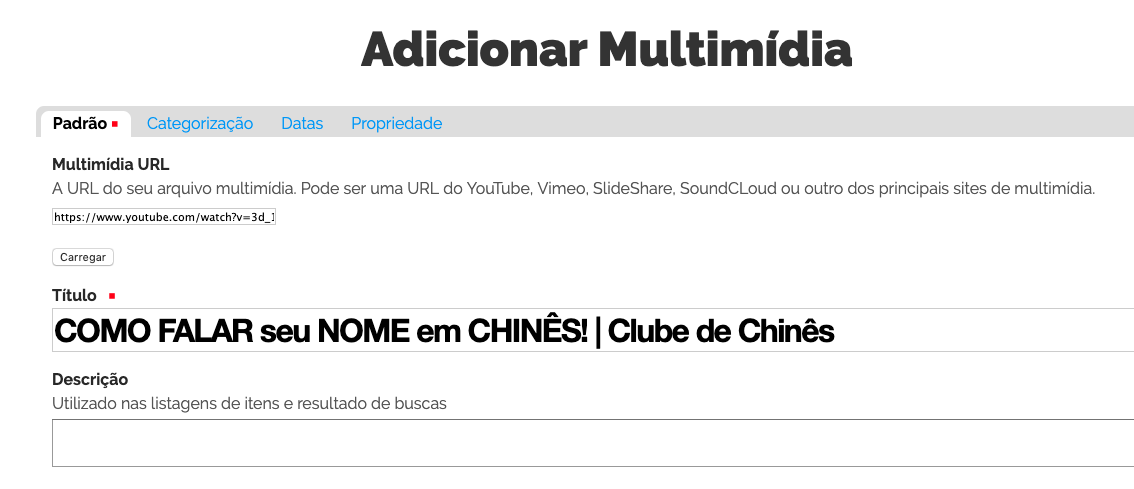
\includegraphics[height=.6\textheight]{./img/001-011_-_embedder.png}
        \caption{\href{https://github.com/collective/sc.embedder}{Embedder}}
    \end{figure}
\end{frame}

\subsection{Agenda}
\begin{frame}
    \frametitle{Agenda}
    \begin{figure}
        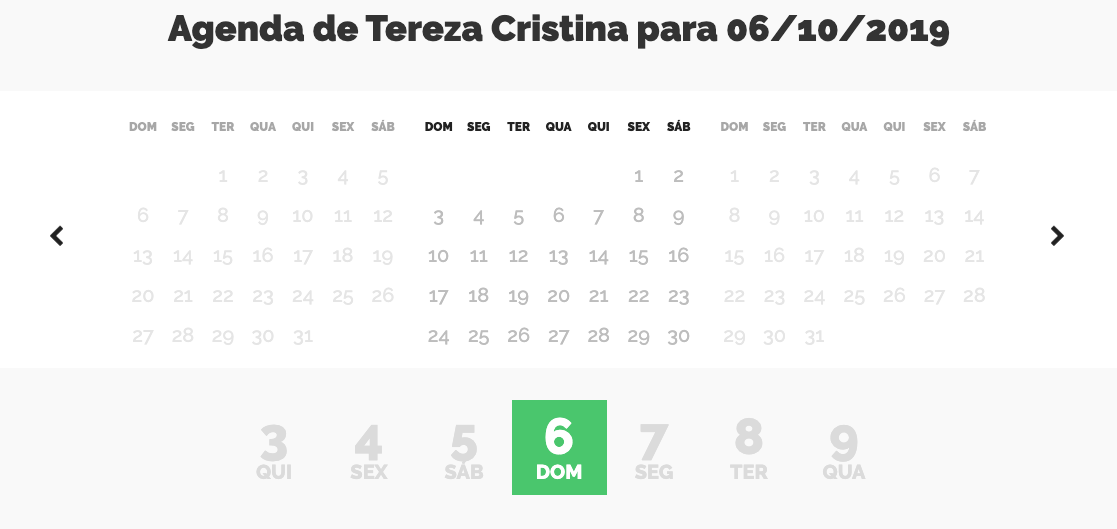
\includegraphics[height=.6\textheight]{./img/001-012_-_agenda.png}
        \caption{\href{https://github.com/plonegovbr/brasil.gov.agenda}{Agenda}}
    \end{figure}
\end{frame}

% \section{Columns example}
% \subsection{Columns example}
% \begin{frame}
%     \frametitle{Columns example}
%     \begin{columns}
%         \column{.5\textwidth}
%         \lipsum[1][1-4]

%         \column{.5\textwidth}
%         \lipsum[2][1-4]
%     \end{columns}
% \end{frame}

% \section{Code example}
% \subsection{Code example}
% \begin{frame}[fragile]
%     \frametitle{Code example}
%     \begin{lstlisting}[language=python]
% @implementer(IBlocksTransformEnabled)
% class View(BrowserView):

%     """Default view, a compose page."""

%     index = ViewPageTemplateFile(
%         'templates/view.pt')

%     def __call__(self):
%         # forbid image indexing as scales are volatile
%         self.request.RESPONSE.setHeader(
%             'X-Robots-Tag', 'noimageindex')
%         return self.index()
%     \end{lstlisting}
% \end{frame}

\end{document}
